\renewcommand{\thesection}{\arabic{section}}  
\renewcommand{\thetable}{\arabic{table}}  
\renewcommand{\thefigure}{\arabic{figure}} 
\renewcommand{\theequation}{\arabic{equation}} 


Standing balance in human everyday environment is often exposed to
unpredictable and continuous external perturbations.  Moreover, when postural
control is impaired or challenged, handrails, canes, and handles are often
used to assist maintaining balance and the effects of these firm supportive
contacts in such conditions should be considered.  Therefore, we examined
changes in postural control in response to continuous, unpredictable
perturbations and explored the effect of using a handle as a supportive
contact.  Postural control of standing subjects was assessed with measurements
of centre of pressure (COP), which we also compared with perturbation waveform
and forces exerted on the handle, to check for correlations.  Kinematic data
were used to determine changes in posture and electromyographic data to define
the magnitude of muscle activity.  The use of handle affected the control of
posture by reducing the excursions of COP.  The reduction was found to be more
reflective in the posterior direction of COP excursions and was also in line
with higher forces exerted on the handle in the same direction.  The change of
posture was immediate when the contact to the handle was omitted and
significantly different between the two conditions.  Muscle activation levels
of the trunk flexor were significantly higher in the hand supported trial.  In
summary, we found that subjects clearly relied on using the handle for
support, even though the perturbations did not pose a significant balance
threat.  Results of direction specific control of posture with hand support
can be considered in rehabilitation and fall prevention programmes.


\section{Introduction}
Postural control is one of the vastly investigated area of human motor control in the last few decades. Most of the research on postural control focused on the role of sensory input in maintaining postural control during quiet standing, and in response to external balance perturbations. However, in our daily lives handrails, canes and handles are often used to assist maintaining balance, since they provide additional supportive contacts with the environment.
With respect to the use of hand contacts for postural control, one of the most investigated phenomena is "light touch" \cite{Jeka1997,Krishnamoorthy2002}. These light, fingertip contacts with stationary objects provide an additional sensory input, which helps individuals to better position them in space \cite{Jeka1997}. Furthermore, a more accurate sensory information improves postural control by reducing the amplitude of the centre of pressure (COP) movement \cite{Jeka1997,johannsen2007effects,Kouzaki2008,Wing2011a}.
However, hand contacts can serve as more than just sensory input. In situations where balance is exposed to larger perturbations, such as experienced on a moving bus or train, a firm hand contact (i.e. holding) is needed, as it provides a much better stabilising potential than a light touch \cite{Maki1997}. Holding to a handle, besides increasing the base of support of a standing individual, also enables generation of forces at the hand to counteract such perturbations \cite{Sarraf2014,Babic2014b}. For this, the location of the handle with respect to the subject’s position is important. Babič et al. \cite{Babic2014b} recently found that handle position relative to the subject, along with support surface perturbation direction and intensity, has a significant effect on the maximal forces exerted at the handle during support surface perturbations in quiet standing. More specifically, lower forces exerted at handles located at shoulder and eye level were needed to maintain a comparable peak displacement of the COP. This indicates that handles were used for postural control irrespective of their position, but certain handle positions could be exploited more efficiently.
Previously mentioned studies all based on discrete perturbations of balance. Such perturbations evoke reactive postural responses and conclusions were made on the basis of these responses. However, a major component of such responses is comprised of motor actions that are related to various sensorimotor reflexes and in less extent to the voluntary component of the postural control [13].
In contrast to discrete perturbations, continuous perturbations involve both reactive and proactive components of motor actions and in this sense offer a complementary insight into the postural control. Therefore, in this research we focused on changes in postural control during continuous perturbations of subject's balance. We aimed to record the mechanical function of the arm in a function of whole body balance stabilization to measure the effect of a firm hand contact on postural control.


\section{Methods}
We measured thirteen healthy right-handed young adults (average age = 22.2 years, SD = 2.2 years, average height 179 cm, SD = 6.2 cm and average weight = 76.7 kg, SD = 8.4 kg). The study was previously approved by the National medical ethics committee (No. 112/06/13) and all subjects participated after giving their written consent. Data of three subjects were  excluded from the analyses due to some technical issues.

\subsection{Experimental protocol}
Subjects were standing on a force plate while their standing balance was being perturbed for 5 minutes by a motorized waist-pull system \cite{Peternel2013} (\FigureAbbr \ref{fig:methods}). They were required to keep upright with their feet placed at hip width, look straight ahead, and maintain balance without making any unnecessary corrective steps. The experiment consisted of two conditions: balancing with ("with handle"; WH) and without ("no handle"; NH) holding onto a handle. In the WH condition subject held onto a stationary handle (diameter $=$ 3.2 cm, length $=$ 12 cm) positioned at shoulder height \cite{Babic2014b} with their right hand. In the NH condition subjects were standing freely with their arms folded across their chest. 
Balance was perturbed using a random white noise signal constructed to emulate mild, daily life perturbations (e.g., public transport) bus and avoid large, abrupt, and startling balance perturbations. This perturbation signal was based on pilot experiments, had a frequency range between 0.25 and 1.00 Hz and the maximum perturbation force of 11\% of the subject's body weight. 
Kinetic data were collected using a force plate (9281CA, Kistler Instrumente AG, Winterthur, Switzerland) under the subjects’ feet and a 3-axis force sensor (45E15A, JR3, Woodland, USA) on the base of the handle, both at 1000 samples/s. Unilateral  (right hand side) kinematic data were collected at a sampling rate of 100 samples/s using a contactless motion capture system (3D Investigator, Northern Digital Inc., Waterloo, Ont., Canada) consisting of a 3$\times$3 camera array. Seven active markers were attached on the subject's right 5th metatarsal-phalangeal, ankle, knee, hip, shoulder, elbow and wrist joint. Electromyographical (EMG) activity of the right leg (Tibialis Anterior; TA, Gastrocnemius lateralis: GA) and of the trunk (Multifidus; MF, Obliques Externus; OE) was measured using Biometrics DataLOG MW8X at a sampling rate of 1000 samples/s. 
Before the start of the experiment, subjects performed three maximal voluntary contractions (MVC) of each of the measured muscles and were exposed to 14 trials of 5 minutes of the WH condition. The aim of these preparatory WH trials was to familiarize the subjects with the experimental set-up and avoid any learning effects observed in previous balance experiments.

\begin{figure}[htb!]
	\centering
	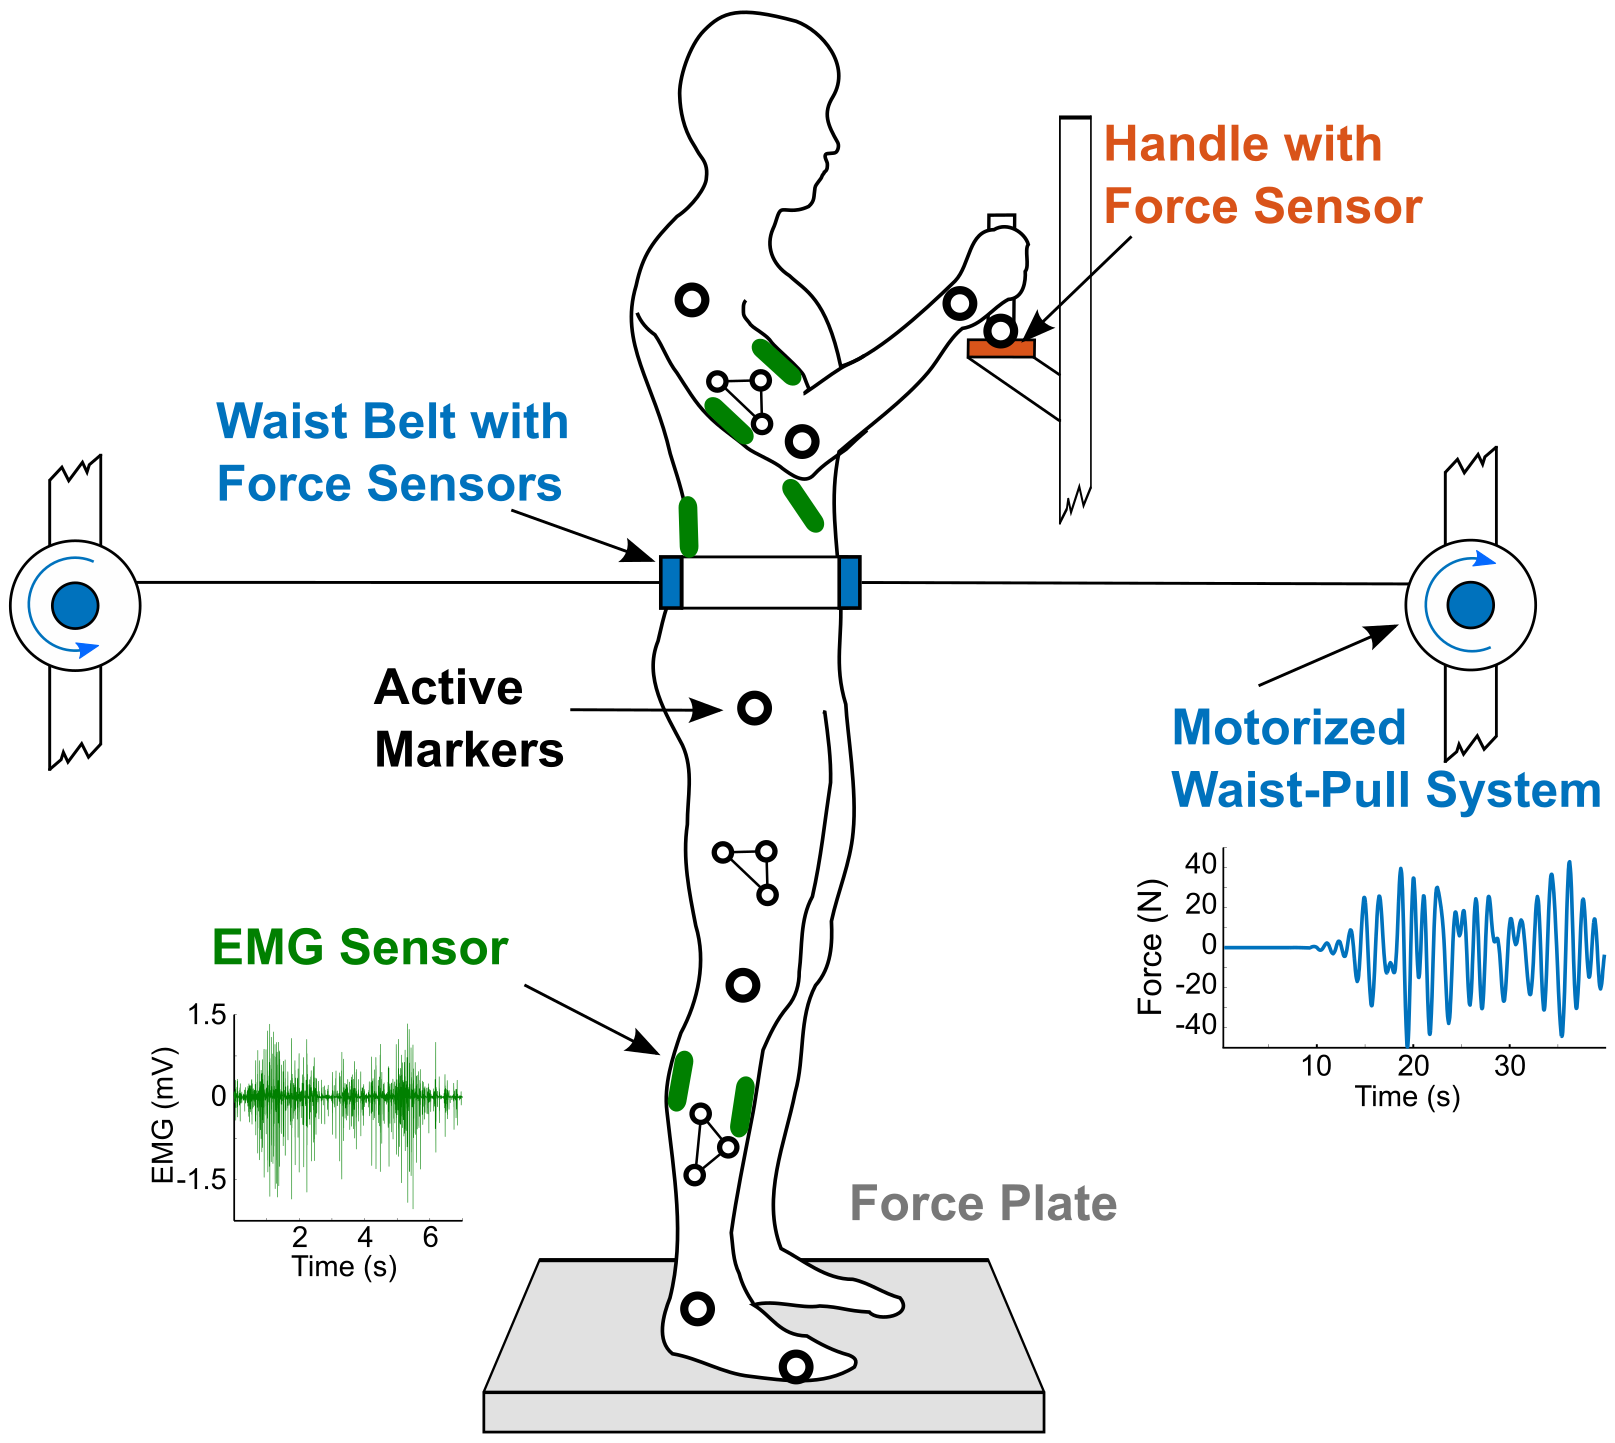
\includegraphics[width=0.85\textwidth]{Jernej/figures/expSetup}
	\caption{\textbf{Experimental setup. }The subject is standing on a force plate, wearing a waist belt connected to the motorized waist-pull system which generated translational force perturbations in the anterior-posterior direction using a random white noise signal constructed to emulate mild, daily life perturbations. The actual perturbation waveform is shown on the plot below the motorized waist-pull system.
			}
	\label{fig:methods}
\end{figure}

\subsection{Data analysis}  
Anteroposterior  displacement of the subject’s centre of pressure (COP) was calculated from the data provided by the force plate on which the subjects were standing. 
Kinematic data were low pass filtered (zero lag, 2nd order Butterworth algorithm, cut-off frequency 20 Hz) \cite{Bartlett1997} and ankle, knee, and hip joint angles were calculated from the joint markers coordinates. 
Mean values of joint angles over time were fitted using an exponential model $y = A^{e-t/\tau} + C$, where $A$ is the gain of the exponential process, $\tau$ is the time constant, $C$ is the offset, and $t$ refers to the trial number) to describe evaluation  of motor adaptation over time \cite{Franklin2003}. The onset of reaching a plateau (adaptation stabilized) was defined by calculating point in time at the three time constants (3$\tau$) of the fitted exponential curve. This is the point when the function reaches a value of less than 5\% of its starting value and was considered as the adaptation stabilized. 
EMG was band-pass filtered (zero lag, 2nd order Butterworth algorithm, with cut-off frequencies of 20 and 450 Hz), full-wave rectified and normalized by division with the MVCs.  By applying a low pass filter (zero lag, 2nd order Butterworth algorithm, 10 Hz cut-off frequency), we created envelopes of EMG signals and then integrated them over time, to observe the accumulated EMG activity.
\subsection{Statistical analysis}
To compare the NH and WH conditions we calculated the average COP displacement, hip, knee, and ankle angles and contact forces exerted on the handle over the 5 minutes for each subject. These individual average values were used for statistical analysis. 
We used paired samples t-test analysis to investigate the differences between the WH and NH conditions and linear correlation to investigate the relationship between the COP displacement and the magnitude of the perturbation (separately for anterior and posterior directions) and between COP and the exerted handle contact force. All statistical analyses were performed using SPSS 21 Inc., Chicago, USA and statistical significance was set at $\alpha =$ 0.05. The effect size (\textit{d}) was calculated by using standard Cohen’s equation ($\hat{d}=\dfrac{\bar{X}_{1} - \bar{X}_{2}}{s}$) \cite{Cohen1988}. 

After comparing the two trials we checked for direction specific differences of COP displacement within each trial. For this, we used a paired samples t-test on averaged measures of anteroposterior COP displacement. The relationship between the perturbation and the COP displacement was investigated in more detail by correlating the perturbation force and COP displacement and by correlating perturbation force and forces on the handle.

\section{Results}
Average anteroposterior displacements of the COP during the NH and WH conditions are shown in \FigureAbbr \ref{fig:cop}. In both conditions COP displacement was larger in the anterior direction (mean $\pm$ SE: NH 38.45 $\pm$ 1.6 mm,  WH 18.15 $\pm$ 1.2 mm) compared to posterior (mean $\pm$ SE: NH $-$34.88 $\pm$ 2 mm, WH $-$11.02 $\pm$ 1.5 mm), but this difference was significant only for the WH condition (\textit{t}(9) $=$ 2.81, \textit{p} $=$ .02, \textit{d} $=$ 1.52). Hence, the remainder of our COP analyses were conducted for the anterior and posterior directions separately. 

Overall, COP displacements were significantly larger in the NH condition compared to WH condition, both in the anterior (difference of 20.3 mm, \textit{t}(9) = 7.78, \textit{p} = .001, \textit{d} = $-$4.15) and posterior direction (difference of 23.9 mm, \textit{t}(9) = $-$11.09, \textit{p} = .001, \textit{d} = $-$3.8). 

\clearpage
As can be seen from \FigureAbbr \ref{fig:corr}A, the correlation between the COP displacement and perturbation force was \textit{r}$_{p} =$ .77 (\textit{p} $<$ .001) and \textit{r}$_{a} =$ .82 (\textit{p} $<$ .001) in the NH condition for the posterior and anterior direction, respectively. For the WH condition (\FigureAbbr \ref{fig:corr}B) the correlations were \textit{r}$_{p} =$ .67 (\textit{p} $<$ .001) and \textit{r}$_{a} =$ .89 (\textit{p} $<$ .001) for the posterior and anterior direction, respectively.

\begin{figure}[!htb]
	\centering
	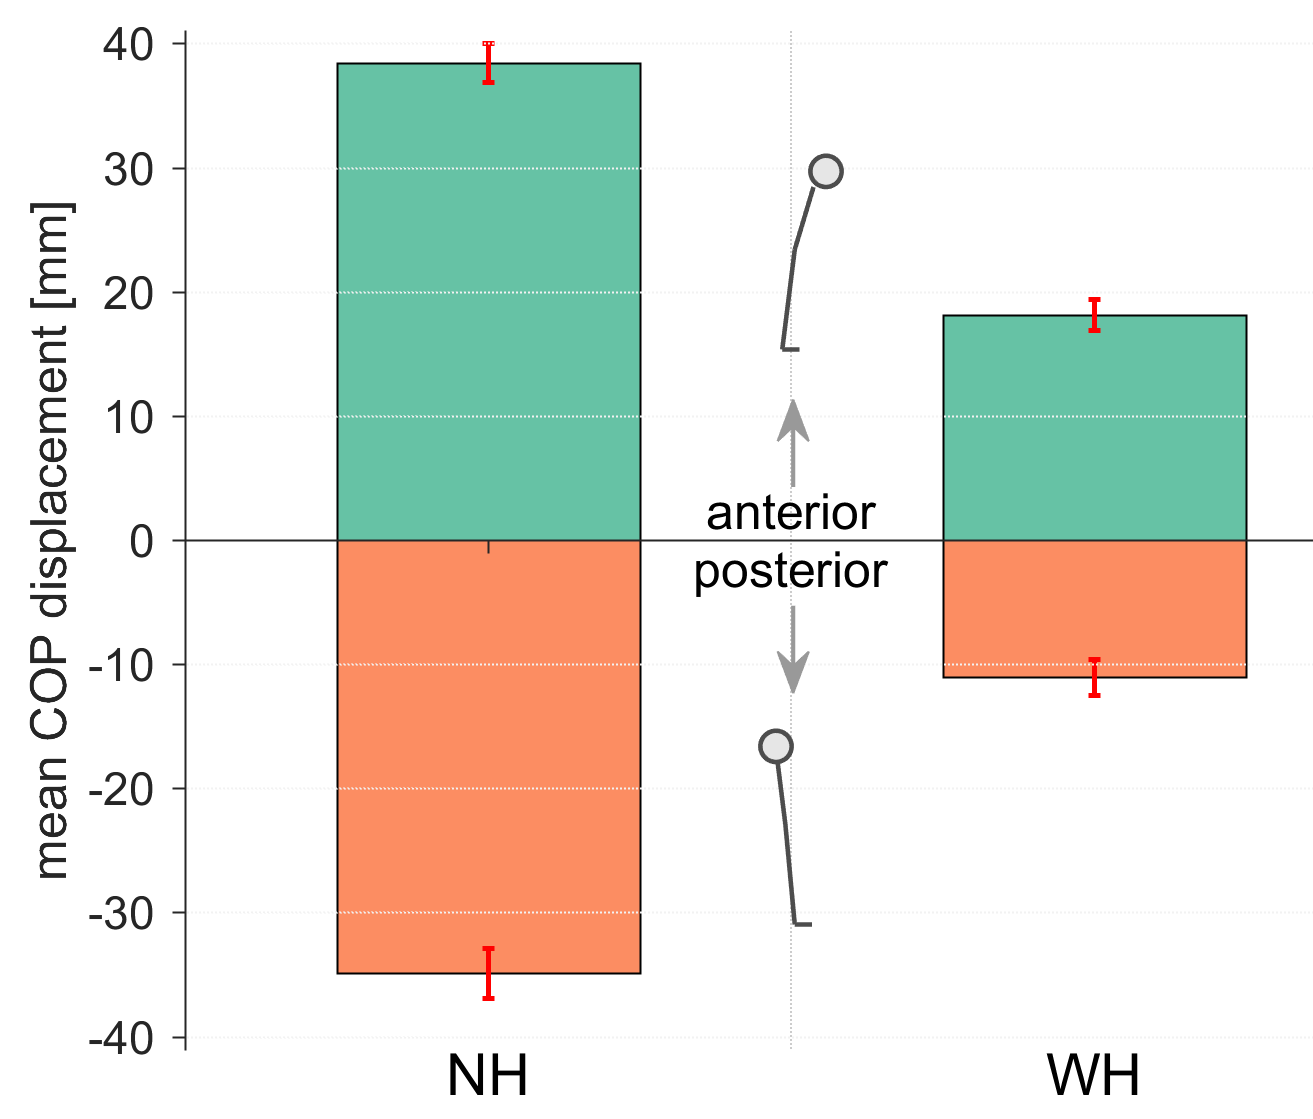
\includegraphics[width=0.7\textwidth]{Jernej/figures/cop}
	\caption{\textbf{Anteroposterior displacement of COP. }Mean COP displacement in NH and WH trials, for the anterior (positive) and posterior (negative) directions. Error bars indicate $\pm$ 1 standard error of the mean.
	}
	\label{fig:cop}
\end{figure}

Correlations between the forces exerted on the handle and the perturbation force (\FigureAbbr \ref{fig:corr}C) were large in both anterior (\textit{r}$_{p}$ $=$ .85, \textit{p} $<$ .001) and posterior direction (\textit{r}$_{a}$ $=$ .81, \textit{p} $<$ .001). However, the slope of a least-squares linear fit to the data indicates, that subjects utilized the handle considerably more for perturbations in the posterior direction (k$_{p}$ = 1.3) than for perturbations in the anterior direction (k$_{a}$ = .86).

\clearpage
\begin{figure}[!htb]
	\centering
	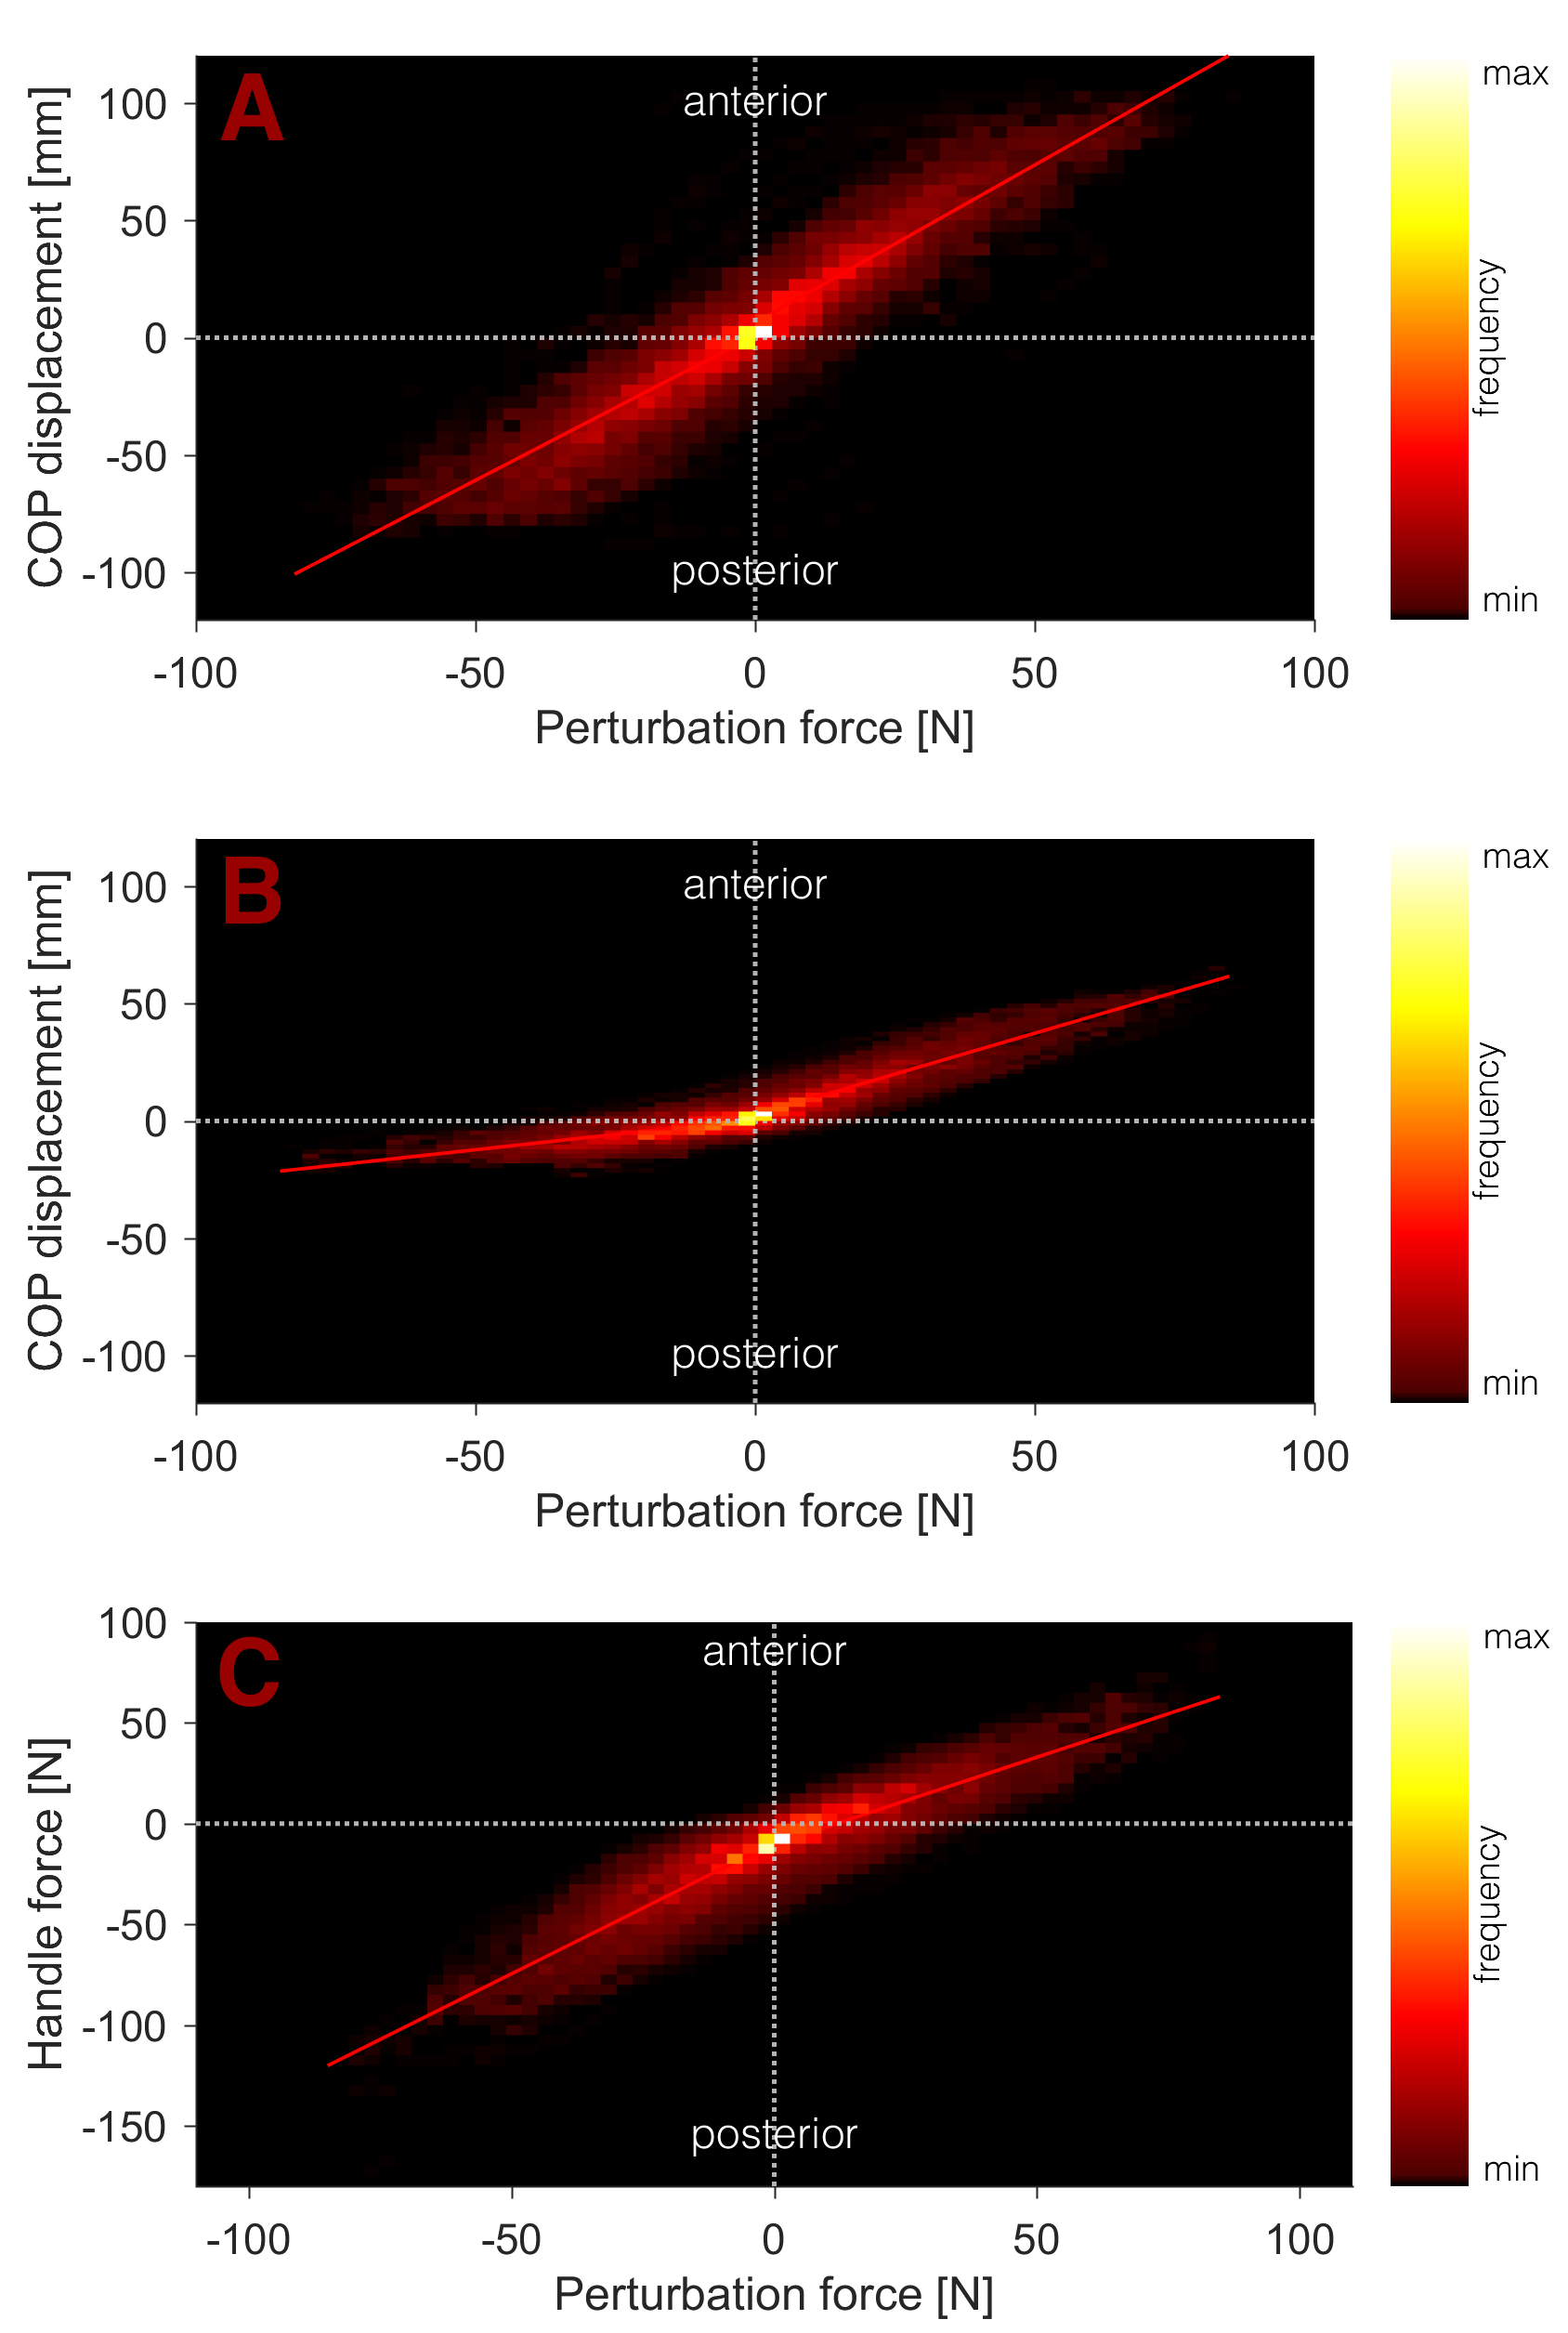
\includegraphics[width=0.7\textwidth]{Jernej/figures/corr}
	\caption{\textbf{Correlation. }\textbf{(A)} Correlation between the perturbation force and COP displacement in the NH condition, \textbf{(B)} correlation between COP displacement and perturbation force in the WH condition, and \textbf{(C)} correlation between handle force and perturbation force in the WH condition.  All correlations were calculated separately for the anterior (positive) and posterior (negative) direction.
	}
	\label{fig:corr}
\end{figure}

Joint angles prior to the start of perturbation were significantly smaller in the NH condition compared to WH condition (\FigureAbbr \ref{fig:jAnglesBars}). Differences were the largest in the knee (mean $\pm$ SE: 169.4 $\pm$ 1.4$^{\circ}$ for NH, 172.9 $\pm$ 1.4$^{\circ}$ for WH, \textit{t}(9) $= -$4.05, \textit{p} $=$ .01, \textit{d} $=$ 1.36 ), followed by the hip (mean $\pm$ SE: 179 $\pm$ 1.8$^{\circ}$ for NH, 181.6 $\pm$ 1.5$^{\circ}$ WH, \textit{t}(9) $= -$2.95, \textit{p} $=$ .024, \textit{d} $=$ 1.13), and ankle (mean $\pm$ SE: 110.4 $\pm$ 1.1$^{\circ}$ for NH, 112.1 $\pm$ 1.2$^{\circ}$ WH, \textit{t}(9) $= -$2.71, \textit{p} $=$ .038, \textit{d} $=$ 1.08).


\begin{figure}[!htb]
	\centering
	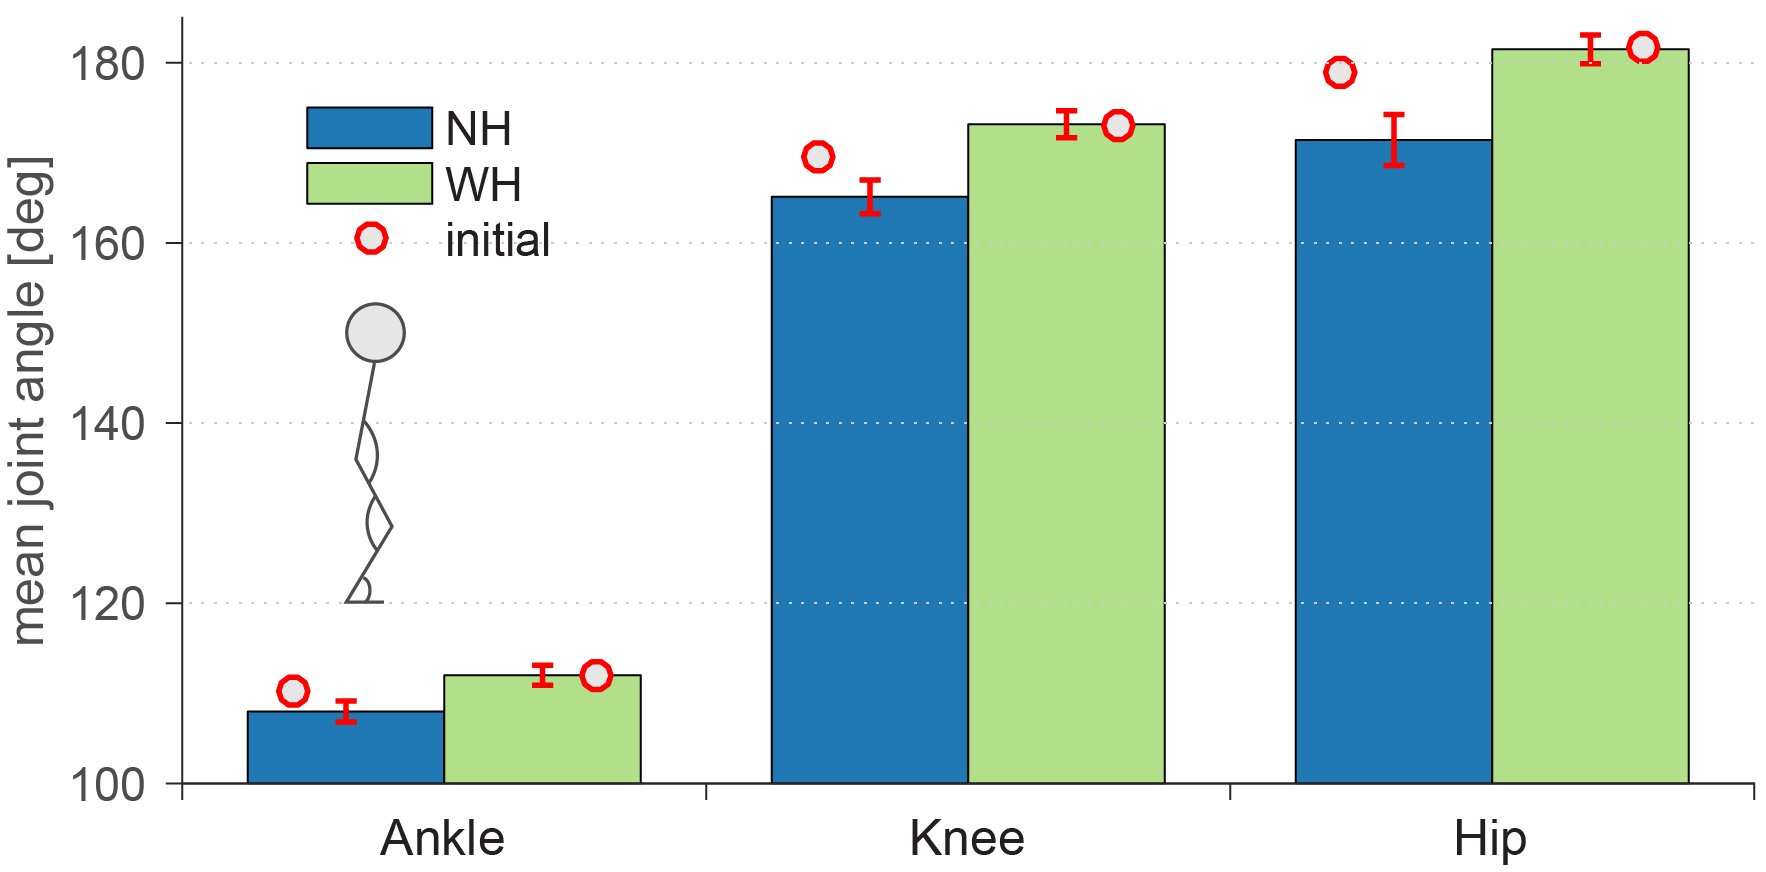
\includegraphics[width=0.7\textwidth]{Jernej/figures/jAnglesBars}
	\caption{\textbf{Ankle, knee and hip joint angles. }Mean value of joint angles during the perturbation is given for NH (blue bars) and WH condition (green bars) and mean joint angles prior to the start of perturbation are shown as red circles above bars. Error bars indicate $\pm$ 1 standard error of the mean.
	}
	\label{fig:jAnglesBars}
\end{figure}

Ankle (A), knee (B), and hip (C) angles over the time course of the perturbation are shown in \FigureAbbr \ref{fig:expFit}. Exponential curves fitted to the data show that mean joint angles in the NH condition changed after the perturbation onset before reaching a steady state. The steady state was reached first by the ankle angle (86 s after perturbation onset), followed by the knee angle (112 s after the perturbation onset) and finally hip angle (195 s after the perturbation onset), resulting in more ankle, knee and hip flexion.

\begin{figure}[!htb]
	\centering
	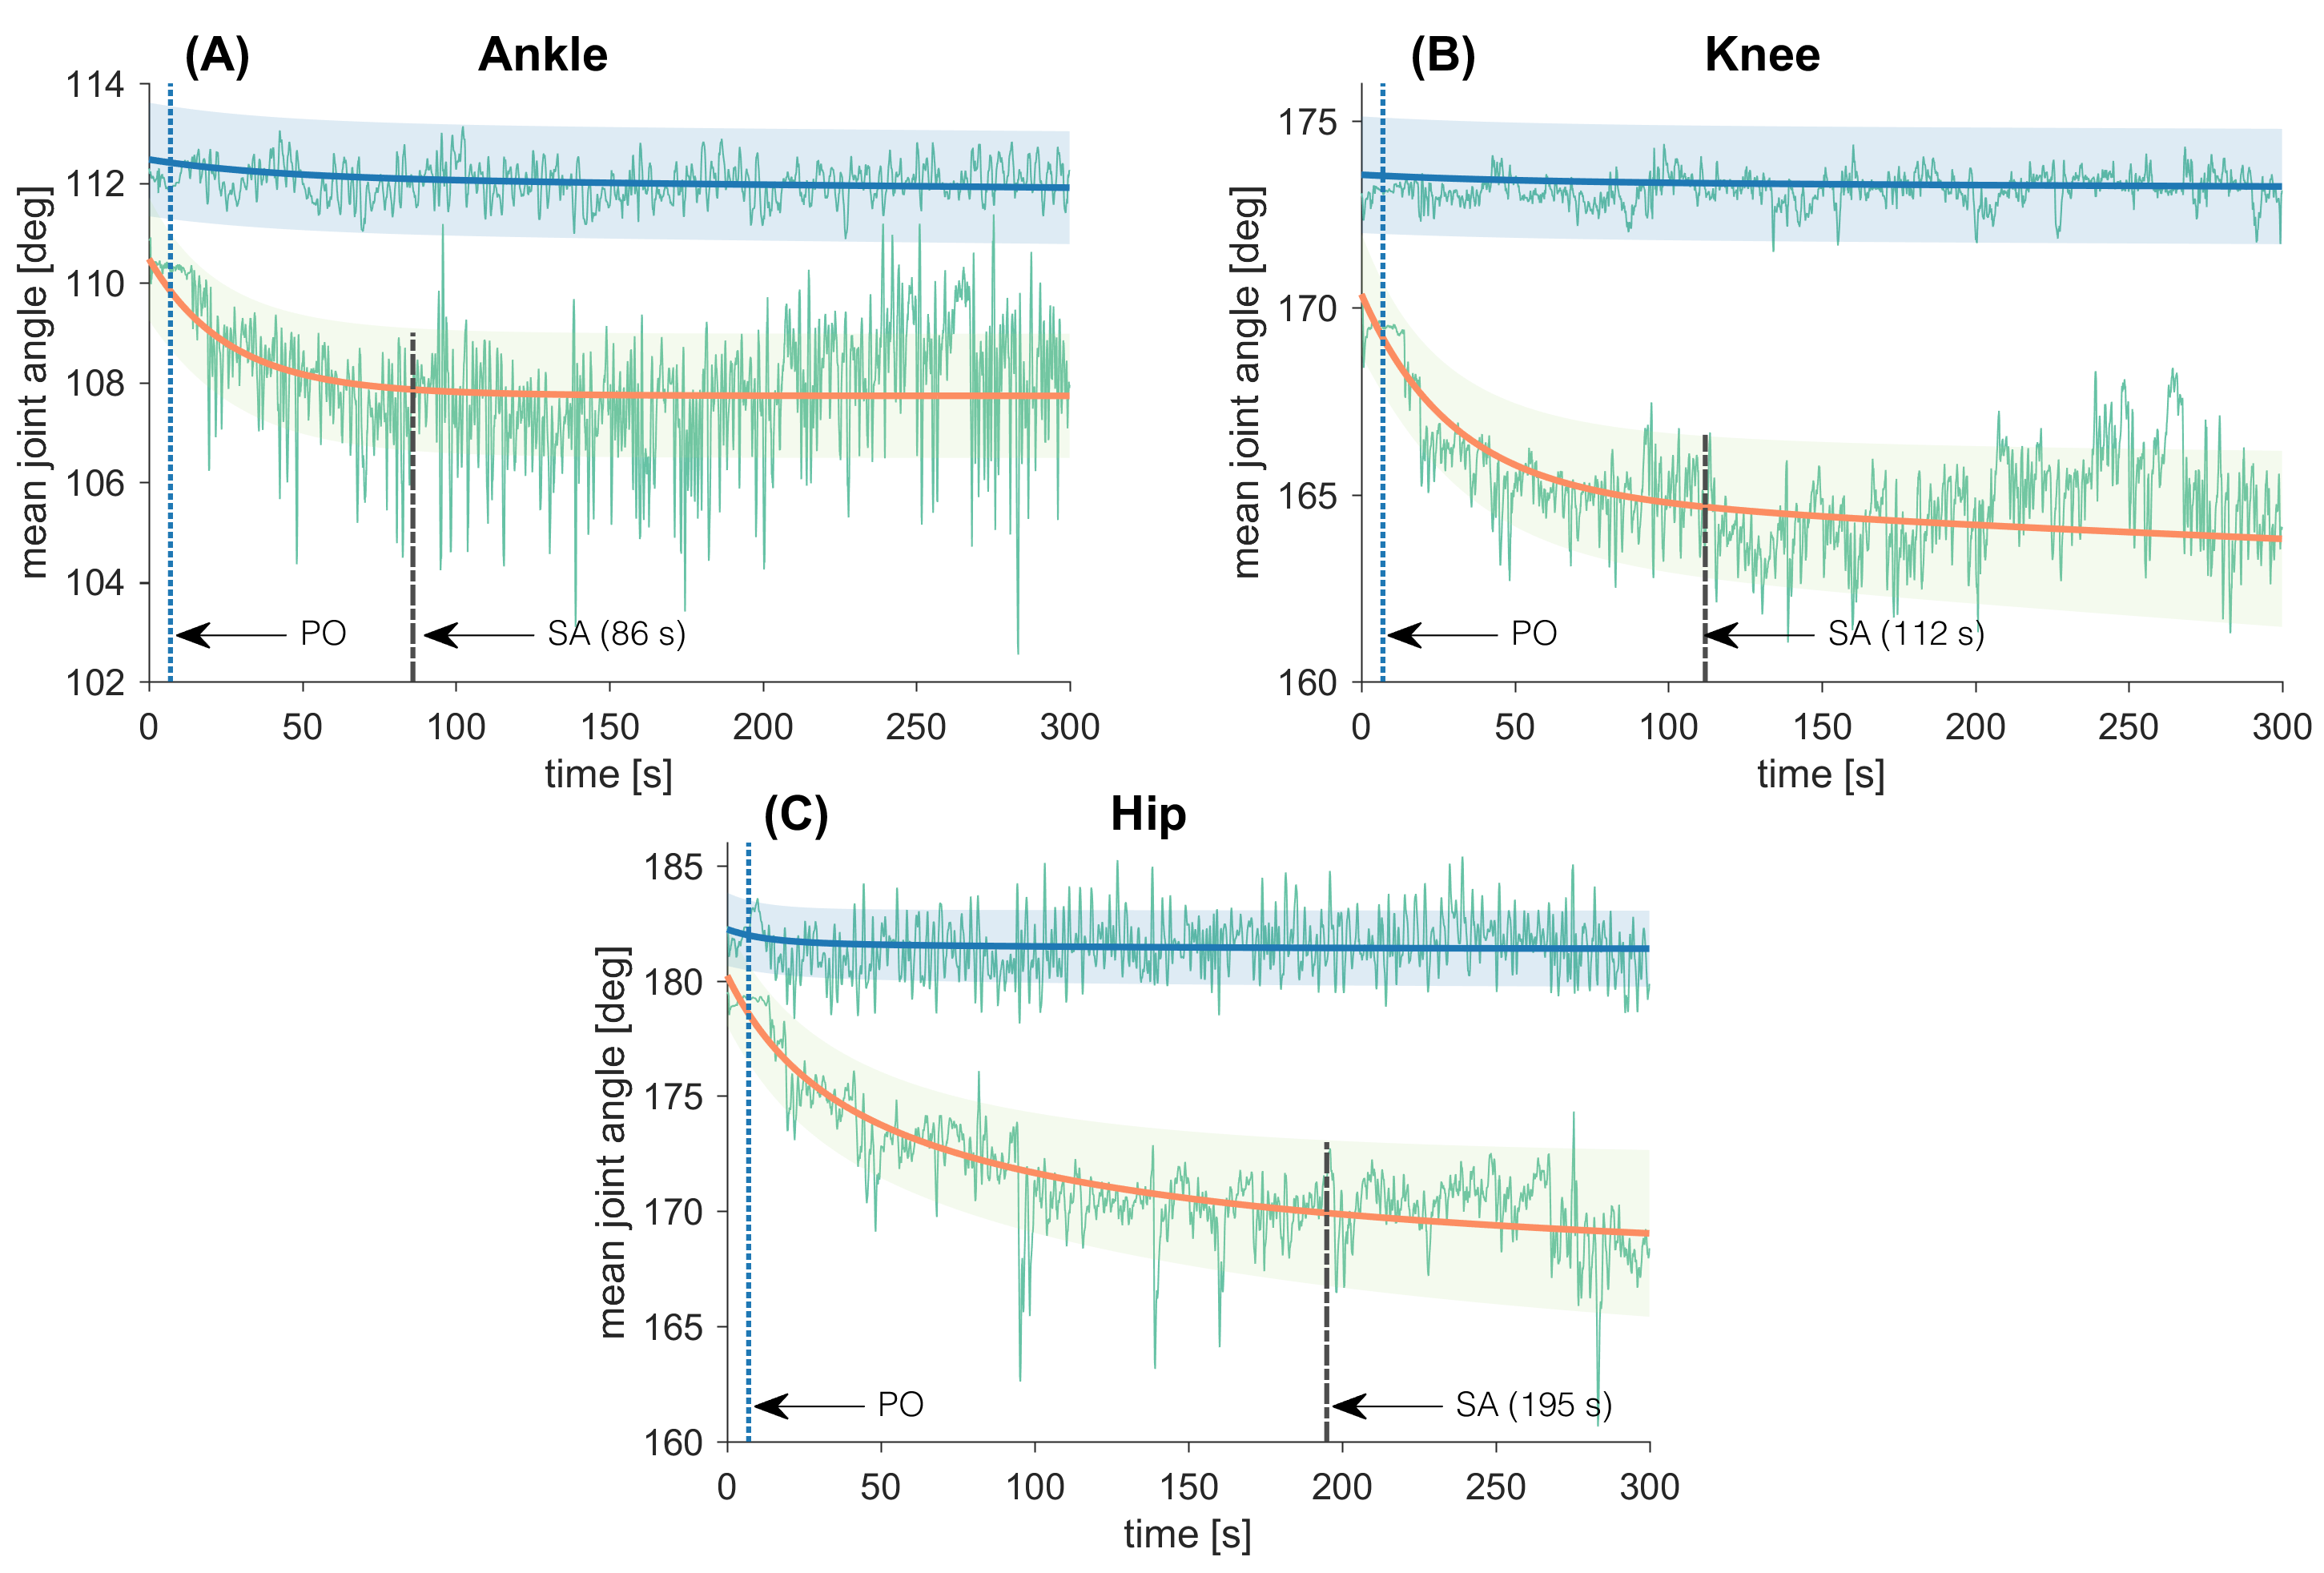
\includegraphics[width=0.92\textwidth]{Jernej/figures/expFit}
	\caption{\textbf{Ankle, knee and hip joint angles. }Figures represent mean ankle \textbf{(A)}, knee \textbf{(B)}, and hip \textbf{(C)} angles over the time course of the perturbation. Thin solid curves represent mean joint angles during NH and WH conditions. Thick solid lines represent exponential curve fit, denoting adaptation of joint angles in the NH (orange) and WH (blue) conditions, while shaded areas represent standard error of the mean. The dotted vertical lines represent perturbation onset (PO) while the dashed vertical lines indicate stabilized changes (adaptation) in the joint angles (SA).
	}
	\label{fig:expFit}
\end{figure}

\clearpage
Finally, muscle activity is significantly lower during the WH condition than during the NH condition both for the leg muscles (GA \textit{t}(9) $=$ 3.57, \textit{p} $=$ .04, \textit{d} $= -$0.89; TA \textit{t}(9) $=$ 6.41, \textit{p} $=$ .002, \textit{d} $= -$1.85) and trunk muscle (MF \textit{t}(9) $=$ 6.5, \textit{p} $=$ .001, \textit{d} $= -$1.01), as can be seen in \FigureAbbr \ref{fig:iemg}. 
Leg muscle activity is lower for 18.4 $\pm$ 4.9\% in the GA (mean $\pm$ SE: NH: 28.97 $\pm$ 6.5\% MVC, WH: 10.6 $\pm$ 2.3\% MVC) and for 23.7 $\pm$ 3.5\% in the TA (mean $\pm$ SE: NH: 27.21 $\pm$ 4\% MVC, WH: 3.47 $\pm$ 1.9\%), while trunk muscle activity is lower for 14.3 $\pm$ 2.1\% in the MF (mean $\pm$ SE: NH: 36.17 $\pm$ 4.5\% MVC, WH: 21.83 $\pm$ 3.7\%).

\begin{figure}[!htb]
	\centering
	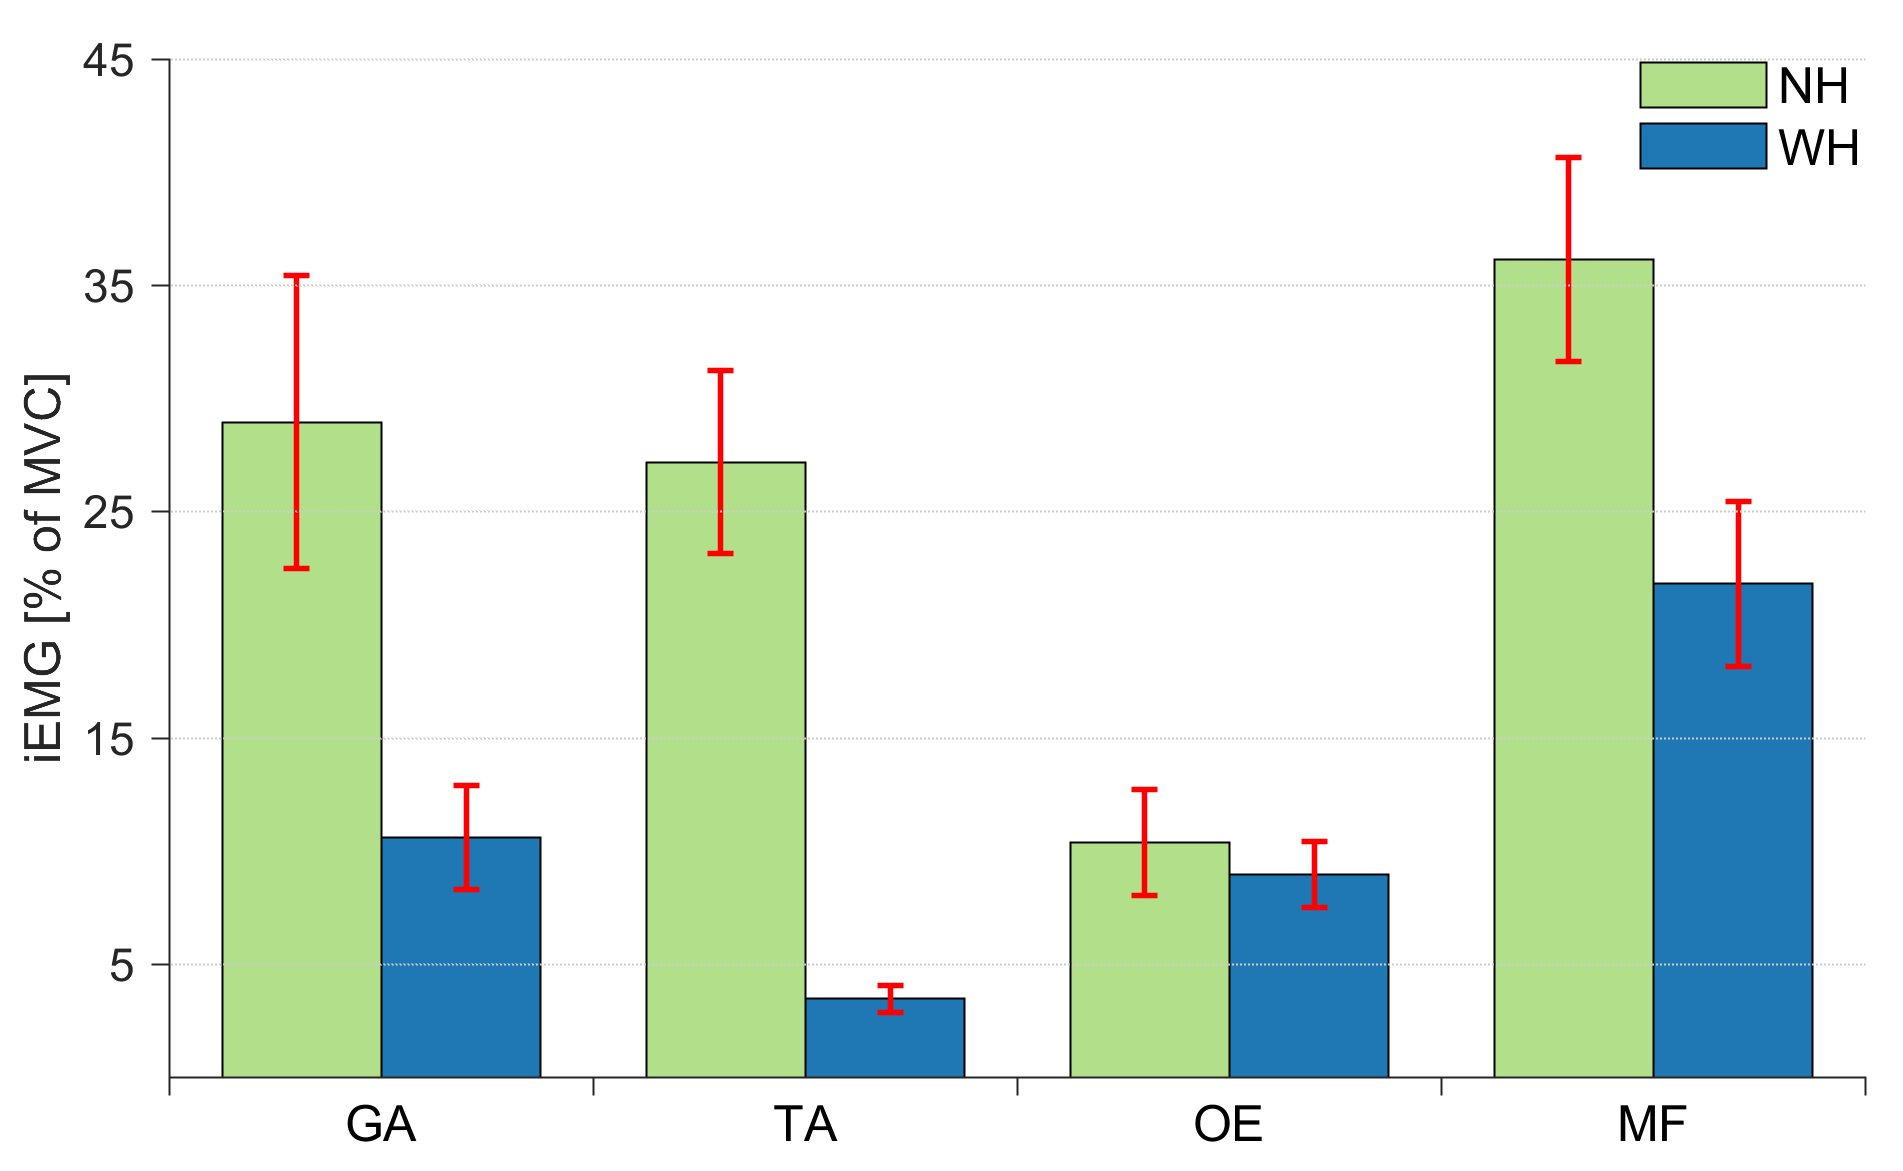
\includegraphics[width=0.7\textwidth]{Jernej/figures/iemg}
	\caption{\textbf{Muscle activity. }Mean integrated EMG activity of leg (GA and TA) and trunk (OE and MF) muscles during the NH (green bars) and WH condition (blue bars). Error bars indicate $\pm$ 1 standard error of the mean.
	}
	\label{fig:iemg}
\end{figure}


\section{Conclusions}
Standing balance in human everyday environment is often exposed to unpredictable and continuous external perturbations. Moreover, when postural control is impaired or challenged, handrails, canes, and handles are often used to assist maintaining balance and the effects of these firm supportive contacts in such conditions should be considered.
Therefore, we examined changes in postural control in response to continuous, unpredictable perturbations and explored the effect of using a handle as a supportive contact. Postural control of standing subjects was assessed with measurements of centre of pressure, which we also compared with perturbation waveform and forces exerted on the handle, to check for correlations. Kinematic data were used to determine changes in posture and electromyographic data to define the magnitude of muscle activity.
COP displacement, hip, knee, and ankle angles, leg and trunk muscle activity and handle contact forces were analysed for the anterior and posterior directions separately, as COP displacement was significantly larger in the anterior direction (WH, 7 mm, \textit{p} $=$ .02). Perturbation force was strongly correlated to COP displacement (all r $>$ .65) and handle forces (r $>$ .8) in both directions. COP displacement was significantly larger in the NH condition compared to WH condition (anterior: 20 mm, posterior: 24 mm, both \textit{p} $=$ .001) and regression indicated that subjects utilized the handle slightly more for posterior perturbations. In the NH condition, all joint angles decreased in anticipation of the perturbation (2-4$^{\circ}$, all \textit{p} $<$ .04) and until 86-195 s following perturbation onset. Finally, leg (18-24\%) and one of the trunk (14\%) muscles increased their activity in the NH condition (all \textit{p} $\leqslant$ .04). 
In summary, we found that subjects clearly relied on using the handle for support, even though the perturbations did not pose a significant balance threat. Results of direction specific control of posture with hand support can be considered in rehabilitation and fall prevention programs.
